\documentclass{article}

\usepackage{graphicx}
\usepackage{physics}
\usepackage{subcaption}
\usepackage{hyperref}
\usepackage{float}

\usepackage[left=2.5cm, right=2.5cm, top=2.5cm, bottom=2.5cm]{geometry}
\setlength{\parindent}{0em}
\setlength{\parskip}{0.8em}

\usepackage{caption}
\captionsetup{width=.9\textwidth}
¨
\usepackage{biblatex}
\addbibresource{report.bib}

\title{Exercise 1, TFY4235 Computational physics}
\author{Martin K. Johnsrud}
\vspace{-8ex}
\date{}

\begin{document}
    \maketitle
    \section*{Introduction}
    The goal of this exercise is to simulate particles as flat, hard disks in a square, 2D container. This is done with a event-driven simulation, as described in the exercise \cite{exercise}. This is implemented in Python, using the built-in library heapq. The simulation is used to first tested with scenarios we know the outcome of, then used to demonstrate the Maxwell-Boltzmann distribution and to investigate the effect of a large, heavy disk hitting a large number of small, inert particles.

    \section*{Implementation}
    The main engine of the code is the function \verb|run_loop()| in \verb|utillities.py|. It follows the algorithm, as laid out in \cite{exercise}, using the objects:
    \begin{itemize}
        \item \verb|particles|, a numpy array with the position and velocity of all the particles.
        \item \verb|t|, a list where \verb|t[i]| is the time of collision number \verb|i|.
        \item \verb|collisions|, a priority queue containing a list for each collision. The list has the time of the collision, the index of the particle(s) involved, and the type of collision it is. The list is sorted by the time of the collision.
        \item \verb|last_collided|, a list of when each particle was involved in a collision.
    \end{itemize}
    The function takes the parameters for the simulation, \verb|(N, T, radii, masses, xi)|, which is resp. the number of particles, number of time steps to be executed, a list with the radii of the particles, a list of the masses, and the restitution coefficient $\xi$. It also takes a function \verb|init|, which is used to set the initial distribution of particles. 
    
    When the particles are initiated, a while loop executes the algorithm as described in \cite{exercise}. The next collision is found by the \verb|heappop| method of \verb| collisions|. The list \verb|last_collided| is used to check if the next collision is valid. The function \verb|exectue_collision| translates the particles forward in time, finds the new velocities for the particles involved in the collision, as shown in ~\cite{exercise}, before finally finding the new collisions, given the updatet positions and velocities. The \verb|run_loop| function can be given the argument \verb|TC=True|. Then, it runs a TC-model, as described in ~\cite{TC}. If the function is passed the argument \verb|condition=func|, it will check the function \verb|func| at regular intervals. This makes it possible to exit the loop early. It is used to run the simulation until $10\%$ of the energy is remaining, as described later in the report.

    The \verb|init| function depends on the situation that is being simulated. To place out particles randomly, in either the whole box or in a smaller box, the \verb|random_dist| function, located in \verb|particle_init.py| is used. This function contains a loop that places a particle randomly within the desired bounds, and gives them velocity with a given magnitude, but uniformly distributed direction. The if the particle overlaps with any of the other particles, already placed it is rejected. There is a "emergency break", if too many particles in a row are rejected, the codes throws an error. As this function only returns an numpy array, the just-in-time compliation library numba is compatible with it. With 2000 particles, of radius 0.008, the \verb|@njit()|-decorator gives a speedup from 15.1 seconds to 0.8 seconds.

    \verb|profile.ipynb| shows the profiling of \verb|run_loop|, and the subroutines that takes the most time. This shows that it is the loop that pushes the next collisions to the priority queue that is the bottle neck. A speedup of about 10 times, for 1000 particles and 10,000 steps was found by rewriting the function that finds the collisions. The notebook \verb|profile_old.ipynb| shows the time used by the old version. The old version of the functions took the index \verb|i| of the particle in question, then found if and when it was to collide with all other collisions, and returned this time as a list. The new version utilizes the fact that everything is contained in numpy-arrays. It does the same operations as the old function, only on arrays instead of single elements. This is done by using masks. An array of booleans can serve as indices, so \verb|lst[np.arange(N) != i]| gives an array with all the elements of \verb|lst[i]|. The profiling show that while most of the time went to the calculation of the next collision, it now goes to pushing to the \verb|collisions|-heap.

    To investigate the creation of craters by a projectile, a function that measures the size of crater is needed. This is done by laying a grid with with a spacing $\Delta x$, looping through each cell to check if there is a particle inside it. The process for checking if a disk is inside each square cell is illustrated in \autoref{check if disk is inside}. Then, the size of the crater is given by $m \Delta x^2$, where $m$ is the number of unoccupied cells. This method relies on choosing a cell size $\Delta x$ large enough so that only cells within the crater are marked as empty. This is done by inspecting the result, and comparing it to a plot of the crater as shown in \ref{crater}.

    To avoid inelastic collapse, the simulation was implemented as at TC-model as described in~\cite{TC}. This is only needed when $\xi<0$, and there are extremely many collisions in a short time step. inelastic collapse were observed when the projectile is approaching the bottom of the box. Good results were found with $t_c = 10^{-8}$.

    \begin{figure}[H]
        \centering
        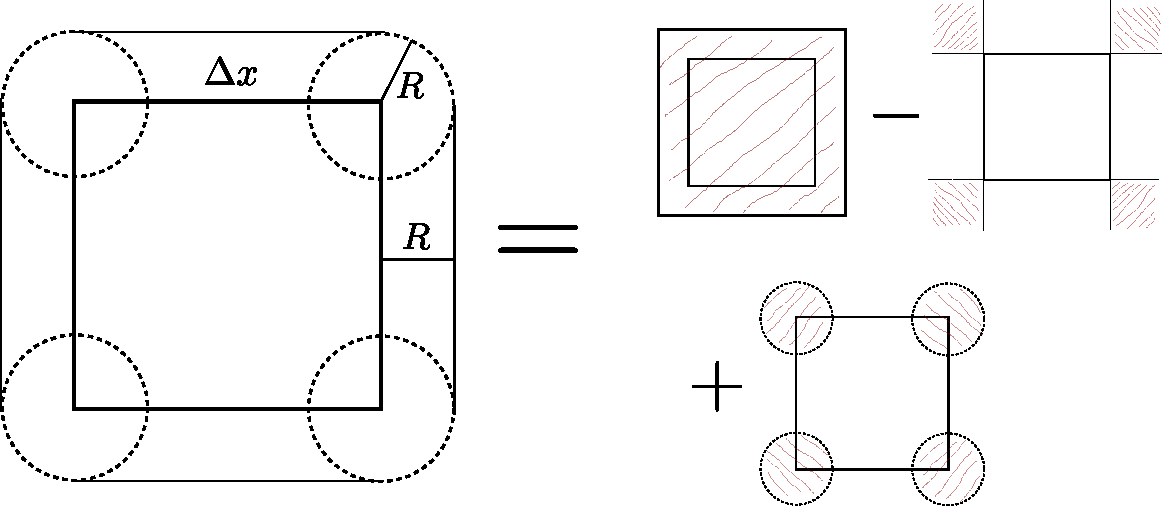
\includegraphics[width=0.8\textwidth]{figure.pdf}
        \caption{Checking if a disk of radius $R$ is inside of a square of side length $\Delta x$, is equivalent to checking if the center of the disk is inside the shape on the left side. Thus, the task is reduced to checking if the center is inside the larger square of side lengths $R + 2 \Delta x$, but not at the corners, or inside one of the circles of radius $R$ centered at the corners of the square.}
        \label{check if disk is inside}
    \end{figure}

    \begin{figure}[H]
        \centering
        \begin{subfigure}{.4\textwidth}                    
            \includegraphics[width=0.7\textwidth]{../plots/problem4/crater0.01.pdf}
            \includegraphics[width=0.7\textwidth]{../plots/problem4/crater0.035.pdf}
        \end{subfigure}
        \begin{subfigure}{.59\textwidth}                    
            \includegraphics[width=0.49\textwidth]{../plots/problem4/particles0.01.pdf}
            \includegraphics[width=0.49\textwidth]{../plots/problem4/particles0.035.pdf}
        \end{subfigure}
        \caption{The grid cells with a particle inside is marked yellow, while the ones without a particle inside, i.e. those counted as making up the grid, are purple. The plot to the right shows the crater.}
        \label{crater}
    \end{figure}


    \section*{Tests}
    Several functions were developed to test the implementation for errors and bugs. First, one particle, starting at in the middle of the box all the way to the left with a velocity with at $45^\circ$ to the $x$-axis, should move in a titled rectangle. With $\xi=1$ it should also conserve energy. \autoref{single particle} shows that this is still the case after $10,000$ events. \autoref{single particle energy} shows that the energy of the system is conserved.
    
    To test the validity of the particle collision, one small, light particle is sent towards a single, large and heavy particle, with varying impact parameter. The relationship between the impact parameter and the escape angle is $s(\theta) = a \cos(\theta / 2)$, where $a$ is the radius of the stationary particle \cite{klasmek}. The result is shown i \autoref{scattering}, and is in good agreement with the theory. Lastly, the energy from a simulation of 2000 particles over 20,000 events is shown in \autoref{test many particles}, together with a snapshot of the particles. The energy is conserved, aside from negligible fluctuations.

    \begin{figure}[H]
        \centering
        \begin{subfigure}{.35\textwidth}
            \centering
            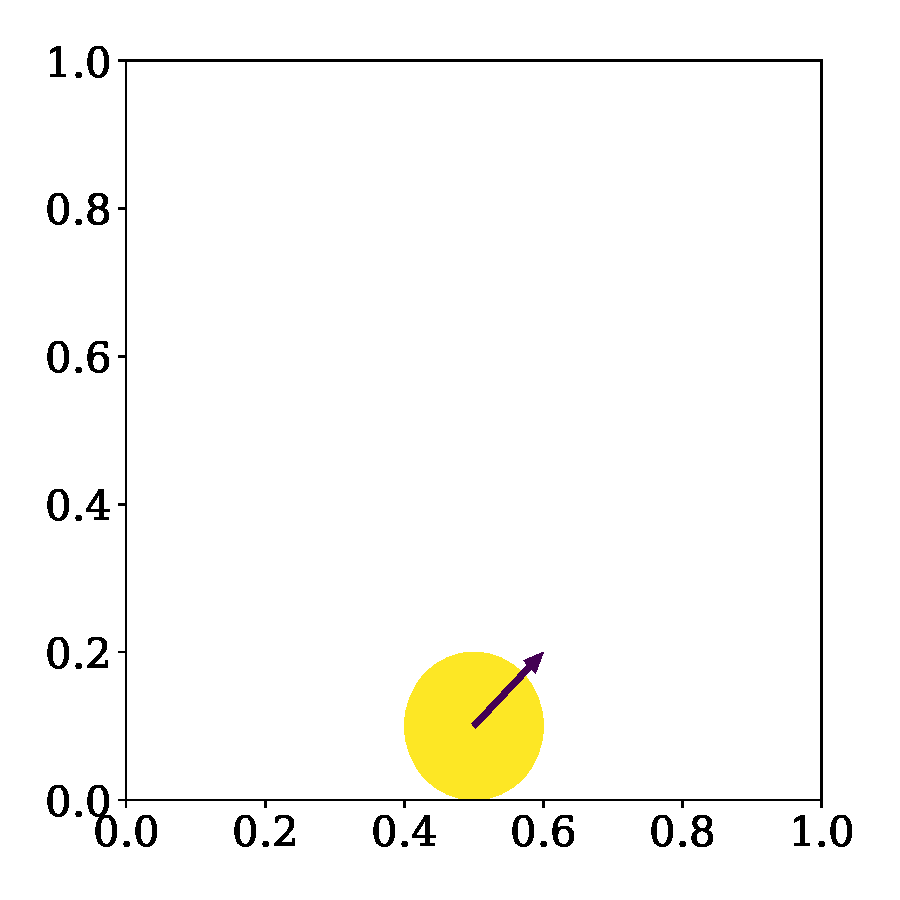
\includegraphics[width=0.49\textwidth]{../plots/test_case_one_particle/particle-4.pdf}
            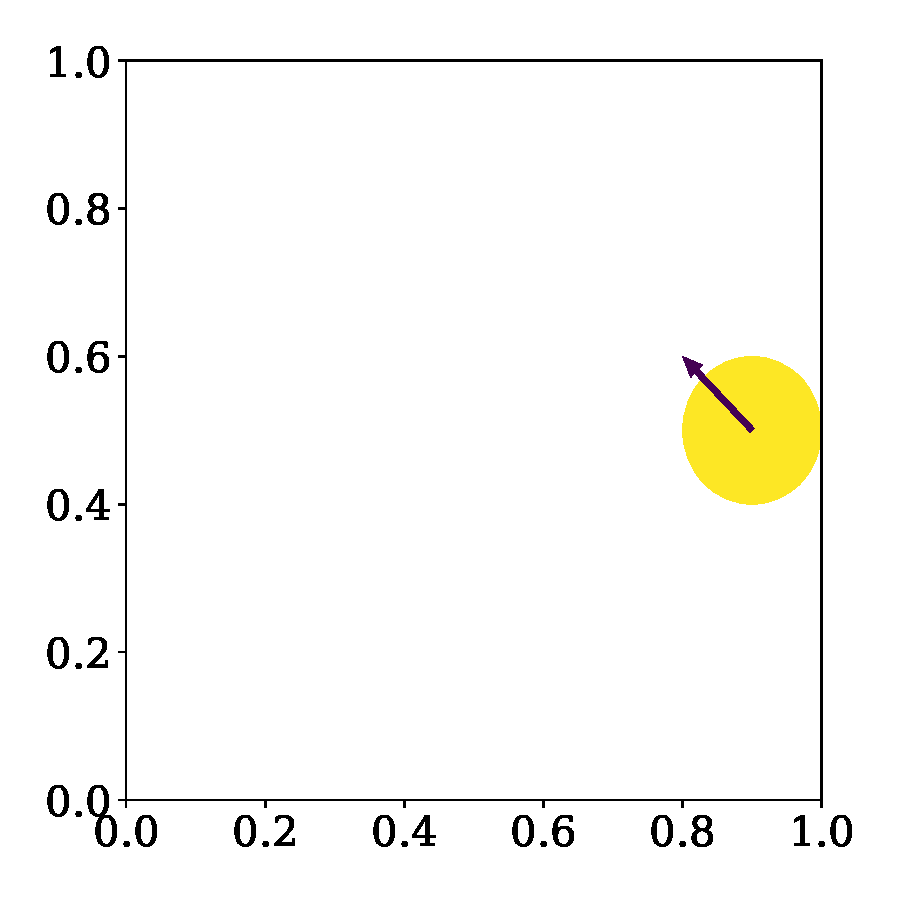
\includegraphics[width=0.49\textwidth]{../plots/test_case_one_particle/particle-3.pdf}
            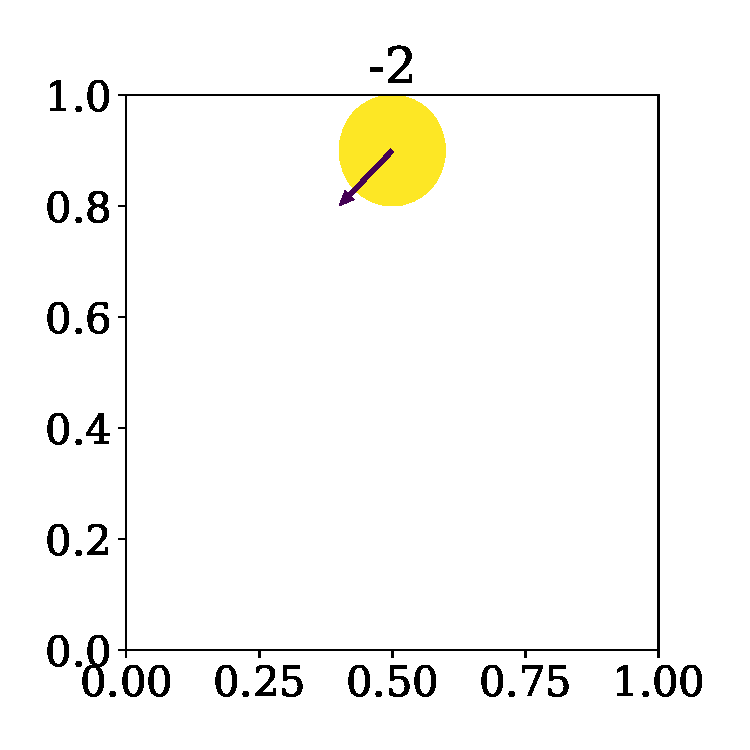
\includegraphics[width=0.49\textwidth]{../plots/test_case_one_particle/particle-2.pdf}
            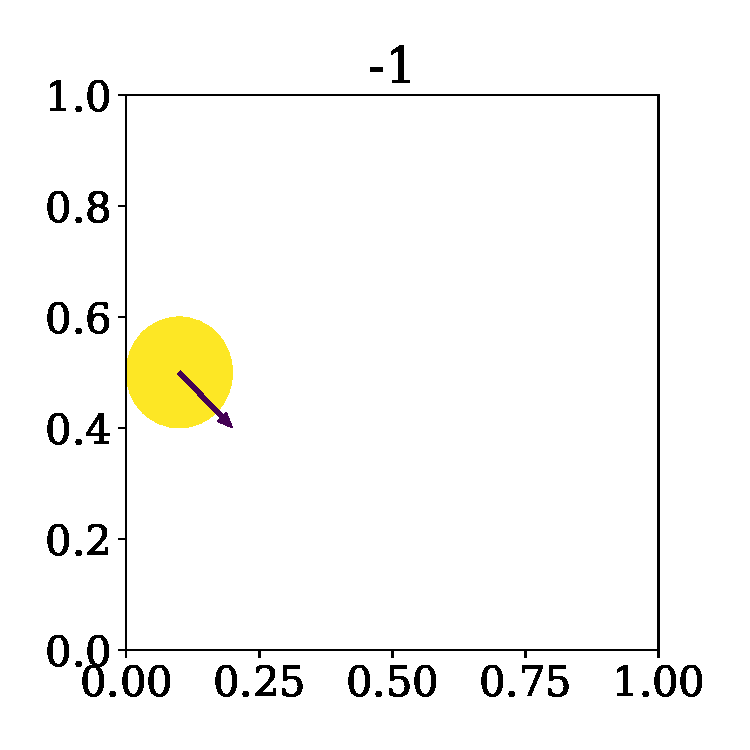
\includegraphics[width=0.49\textwidth]{../plots/test_case_one_particle/particle-1.pdf}
            \caption{After $10 000$ steps, the disk still follows a regular pattern}
            \label{single particle}
        \end{subfigure}
        \begin{subfigure}{.64\textwidth}
            \centering
            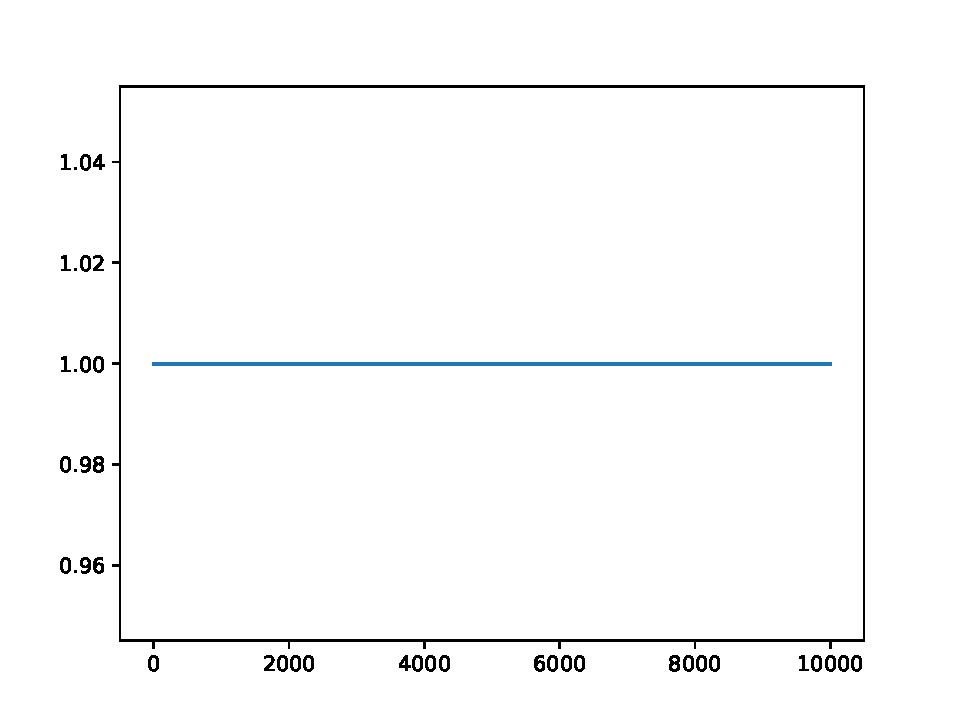
\includegraphics[width=.8\textwidth]{../plots/test_case_one_particle/energy.pdf}
            \caption{The energy of a single particle is constant.}
            \label{single particle energy}
        \end{subfigure}
    \end{figure}

    \begin{figure}[H]
        \centering
        \hspace{-10mm}
        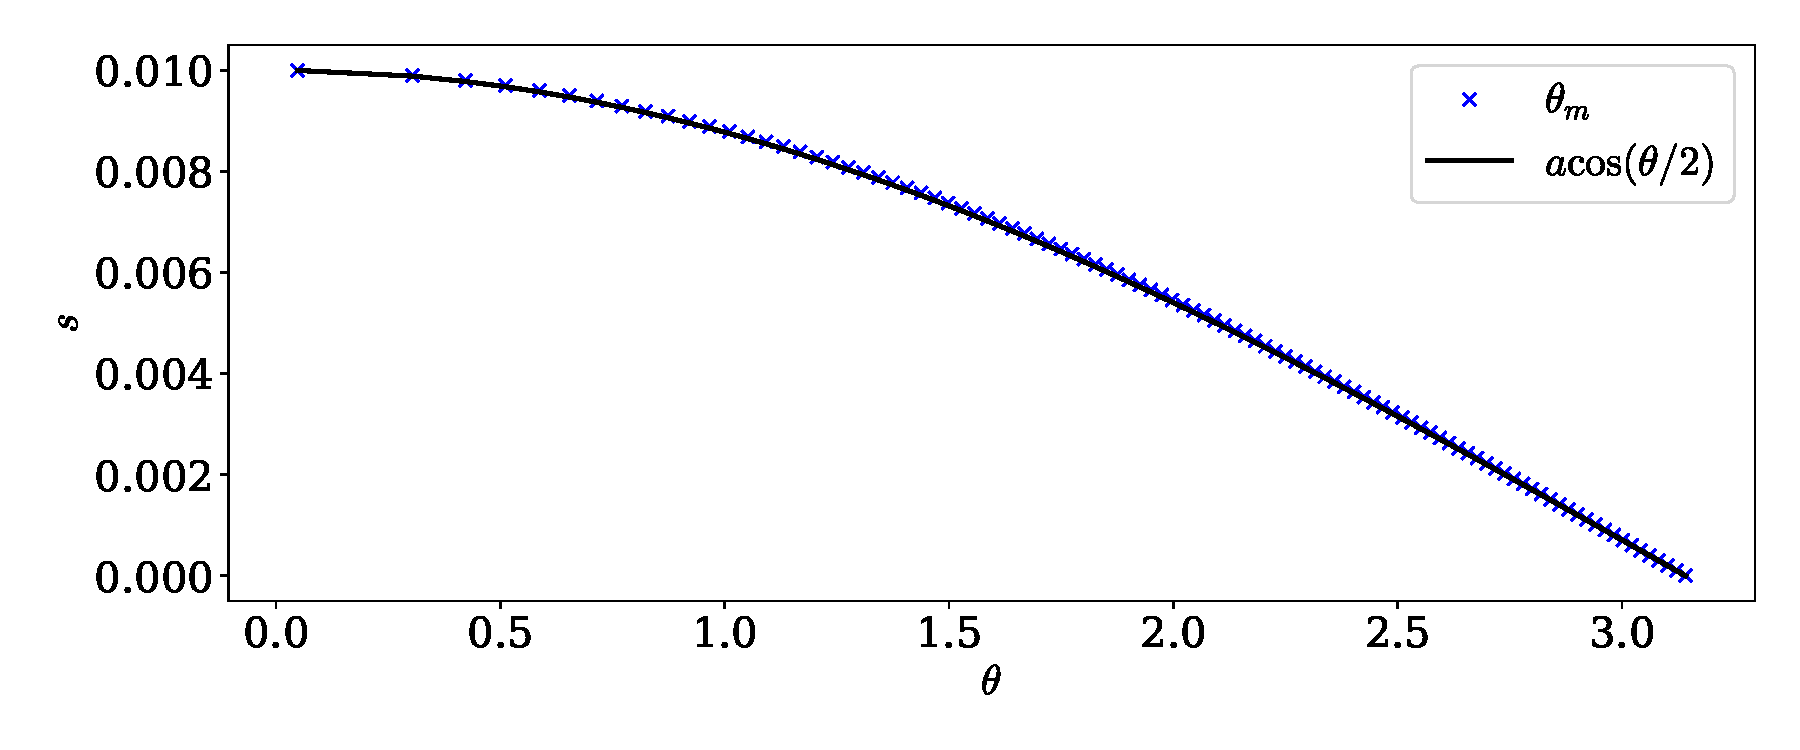
\includegraphics[width=0.7\textwidth]{../plots/test_case_collision_angle/collision_angle.pdf}
        \caption{The impact parameter $S$, as a function of scattering angle. The dashed lines are the theoretical values, $\theta_m$ are the values from the simulation.}
        \label{scattering}
    \end{figure}

    \begin{figure}[H]
        \centering
        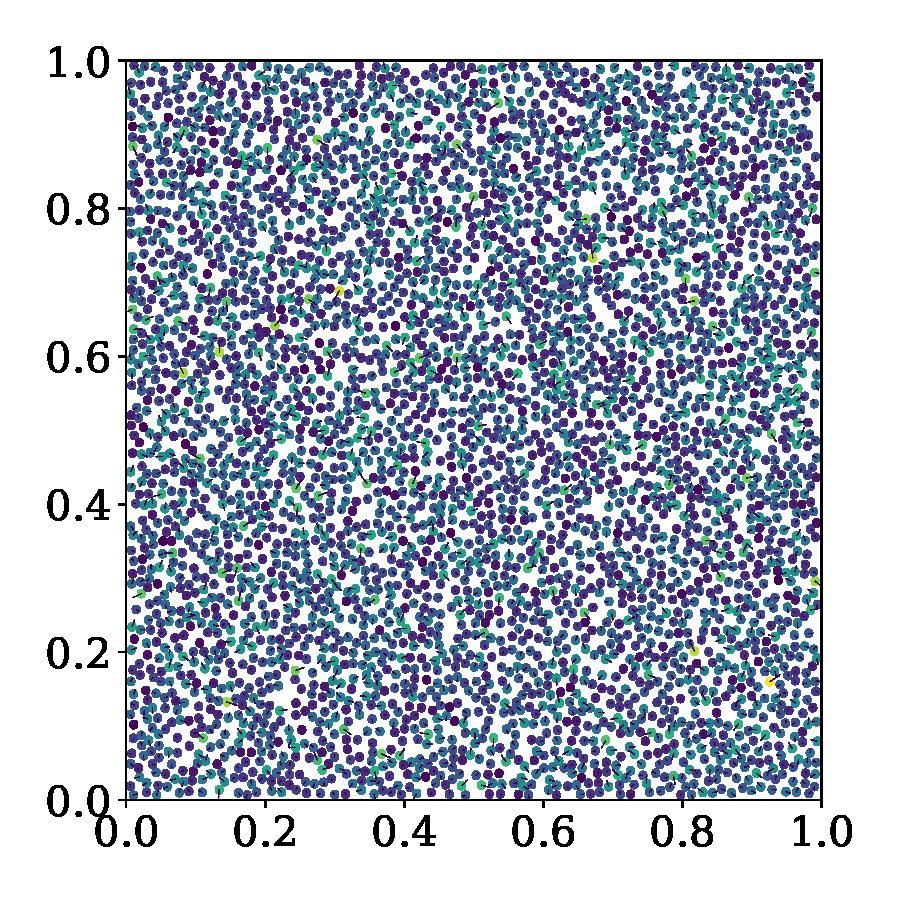
\includegraphics[width=0.35\textwidth]{../plots/test_case_many_particles/test_case_many_particles.pdf}
        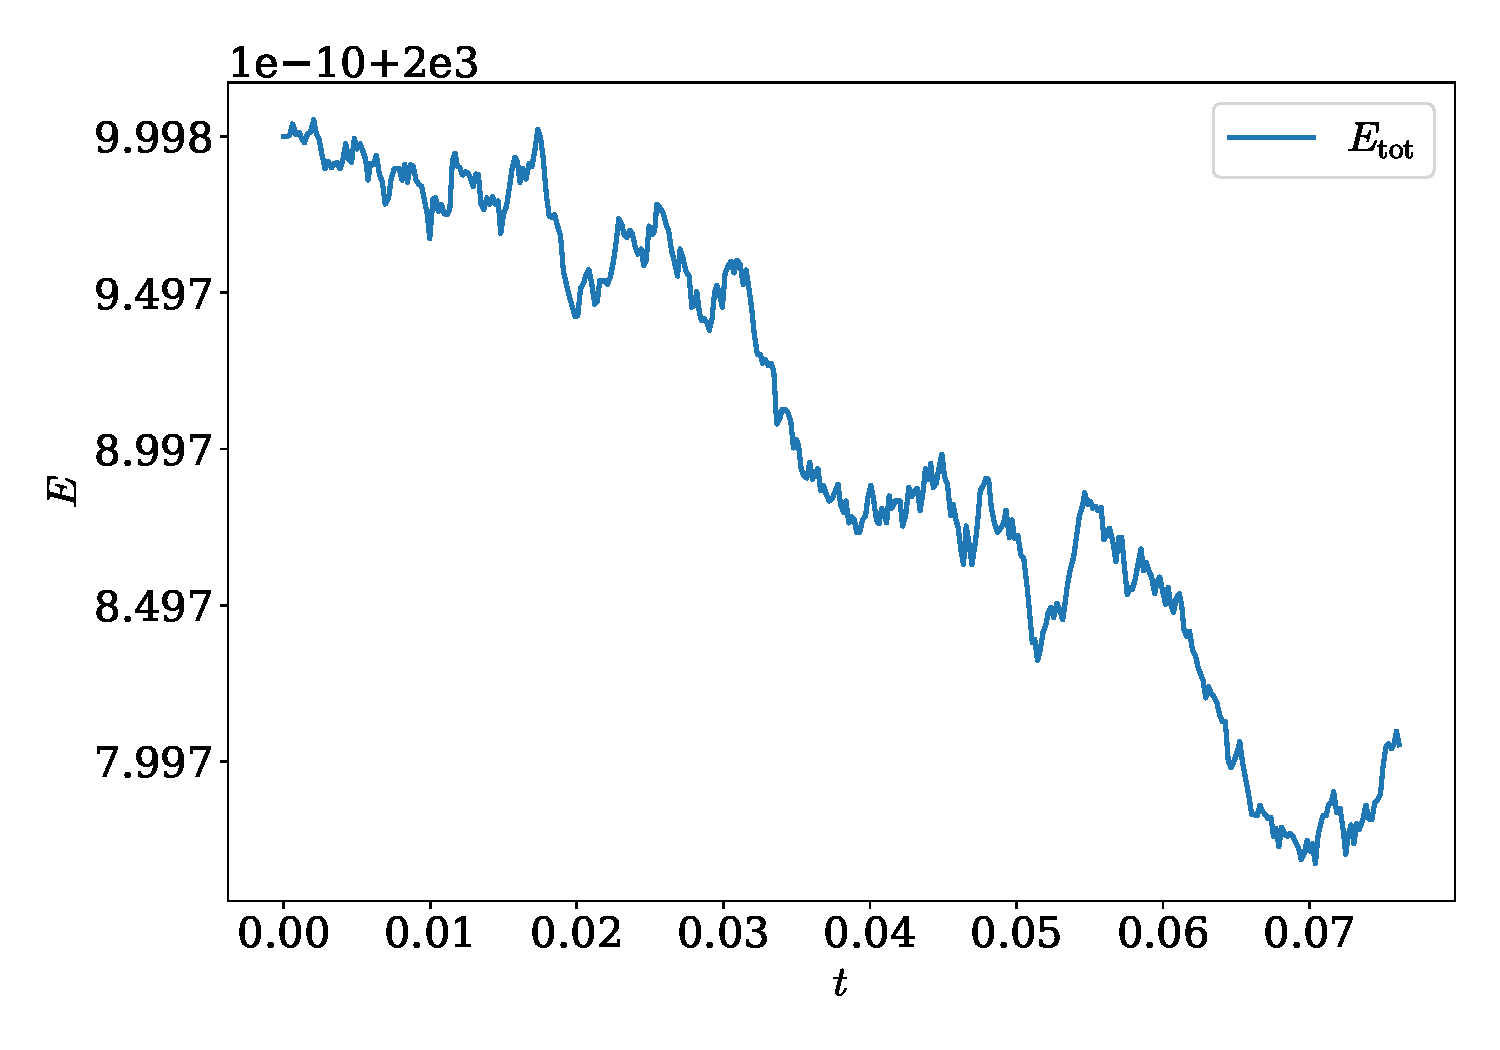
\includegraphics[width=0.54\textwidth]{../plots/test_case_many_particles/energy.pdf}
        \caption{On the left is a snapshot of the particles. The arrows represent the velocities. On the right, the energy is plotted as a function of events. The energy loss can be seen to be negligible.}
        \label{test many particles}
    \end{figure}

    \section*{Results}
    \subsection*{Velocity distribution}

    When the system is first initiated, all particles have the same magnitude of velocity. As the system equilibrates, it should reach the Maxwell-Boltzmann distribution, which in 2D is
    \begin{equation*}
        f(v) = \frac{m v}{T} \exp \left(-\frac{m v^2}{2 T}\right),
    \end{equation*}
    when using units in which $k_b = 1$. The equipartition theorem gives the temperature $T = E$ in 2D. \autoref{problem1 av vel} shows the average velocity as a function of time. It is a indication of when the system has reached equilibrium, and was used to find a good point to start sampling. After that, the simulation is sampled every $N$ event, where $N$ is the number of particles. This ensures somewhat independent samples. \autoref{problem1 dist} shows the velocity distribution, compared to the Maxwell Boltzmann distribution.

    \begin{figure}[H]
        \centering
        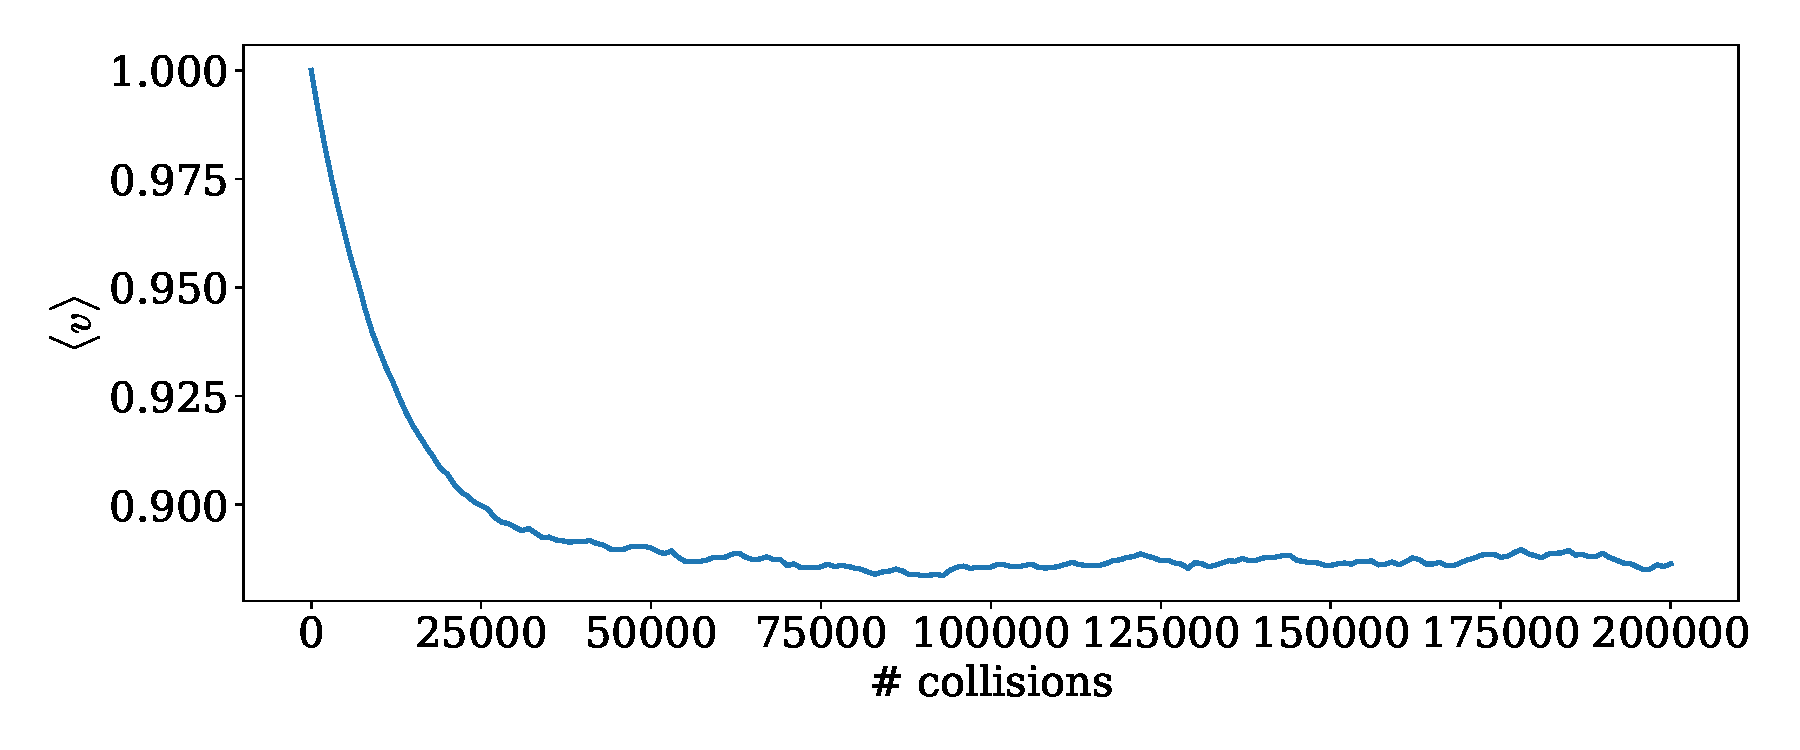
\includegraphics[width=0.8\textwidth]{../plots/problem1/v_av.pdf}
        \caption{Average velocity, as a function of collisions. The distribution reaches equilibrium around $6000$ collisions, or $3N$}
        \label{problem1 av vel}
    \end{figure}
    
    \begin{figure}[H]
        \centering
        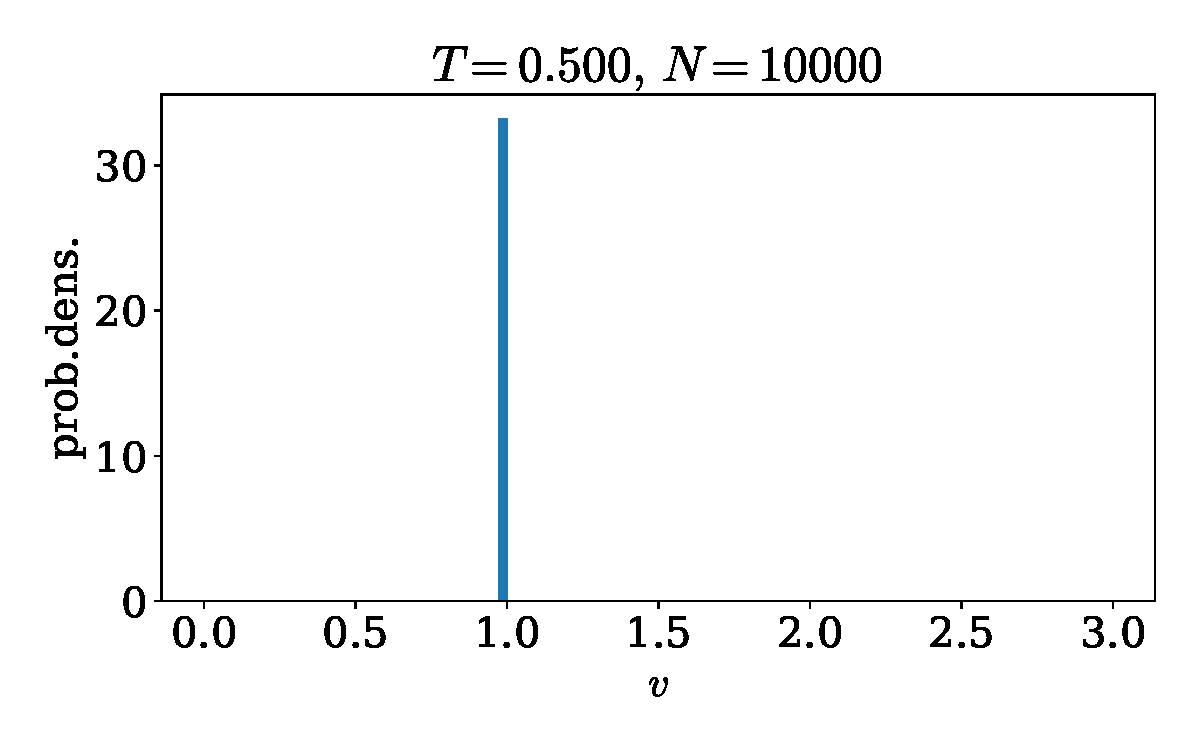
\includegraphics[width=0.49\textwidth]{../plots/problem1/2/vel_dist.pdf}
        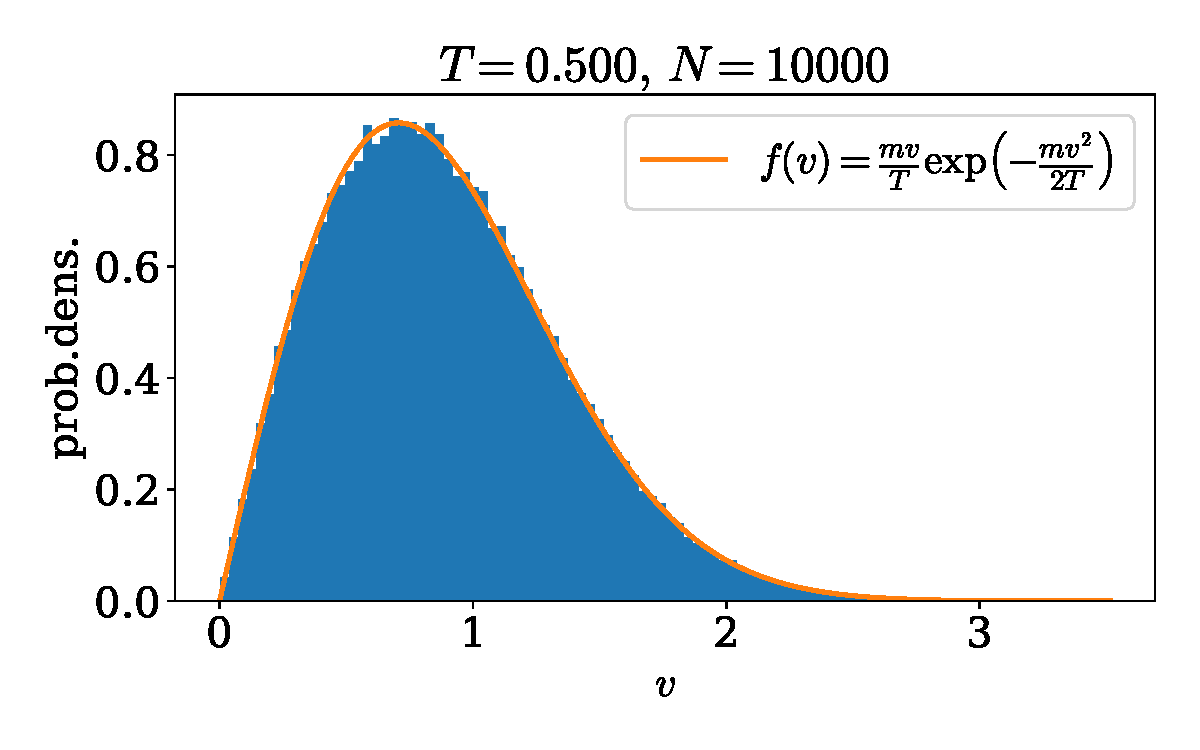
\includegraphics[width=0.49\textwidth]{../plots/problem1/vel_dist.pdf}
        \caption{The velocity distribution is a good fit with the Maxwell-Boltzmann distribution, shown as a blue line.}
        \label{problem1 dist}
    \end{figure}

    Next, two different types of particles are simulated, one with a mass of $1$, the other with a mass of $4$. As the particles have the same magnitude of velocity, but different masses, they will have different energies, and thus have different energies (although temperature is in fact only defined in equilibrium). \autoref{problem2 av vel} shows how the average speed evolves over time. After the system equilibrates, the both sets of particles should reach the Maxwell-Boltzmann distribution with a common temperature. The peak will nonetheless be at different velocities. This is, however, only the case when the restitution coefficient $\xi$ is set to 1. For values less than one, the two sub systems approach each other in temperature, but does not come into equilibrium, as shown in \autoref{problem2 av en}.

    \begin{figure}[H]
        \centering
        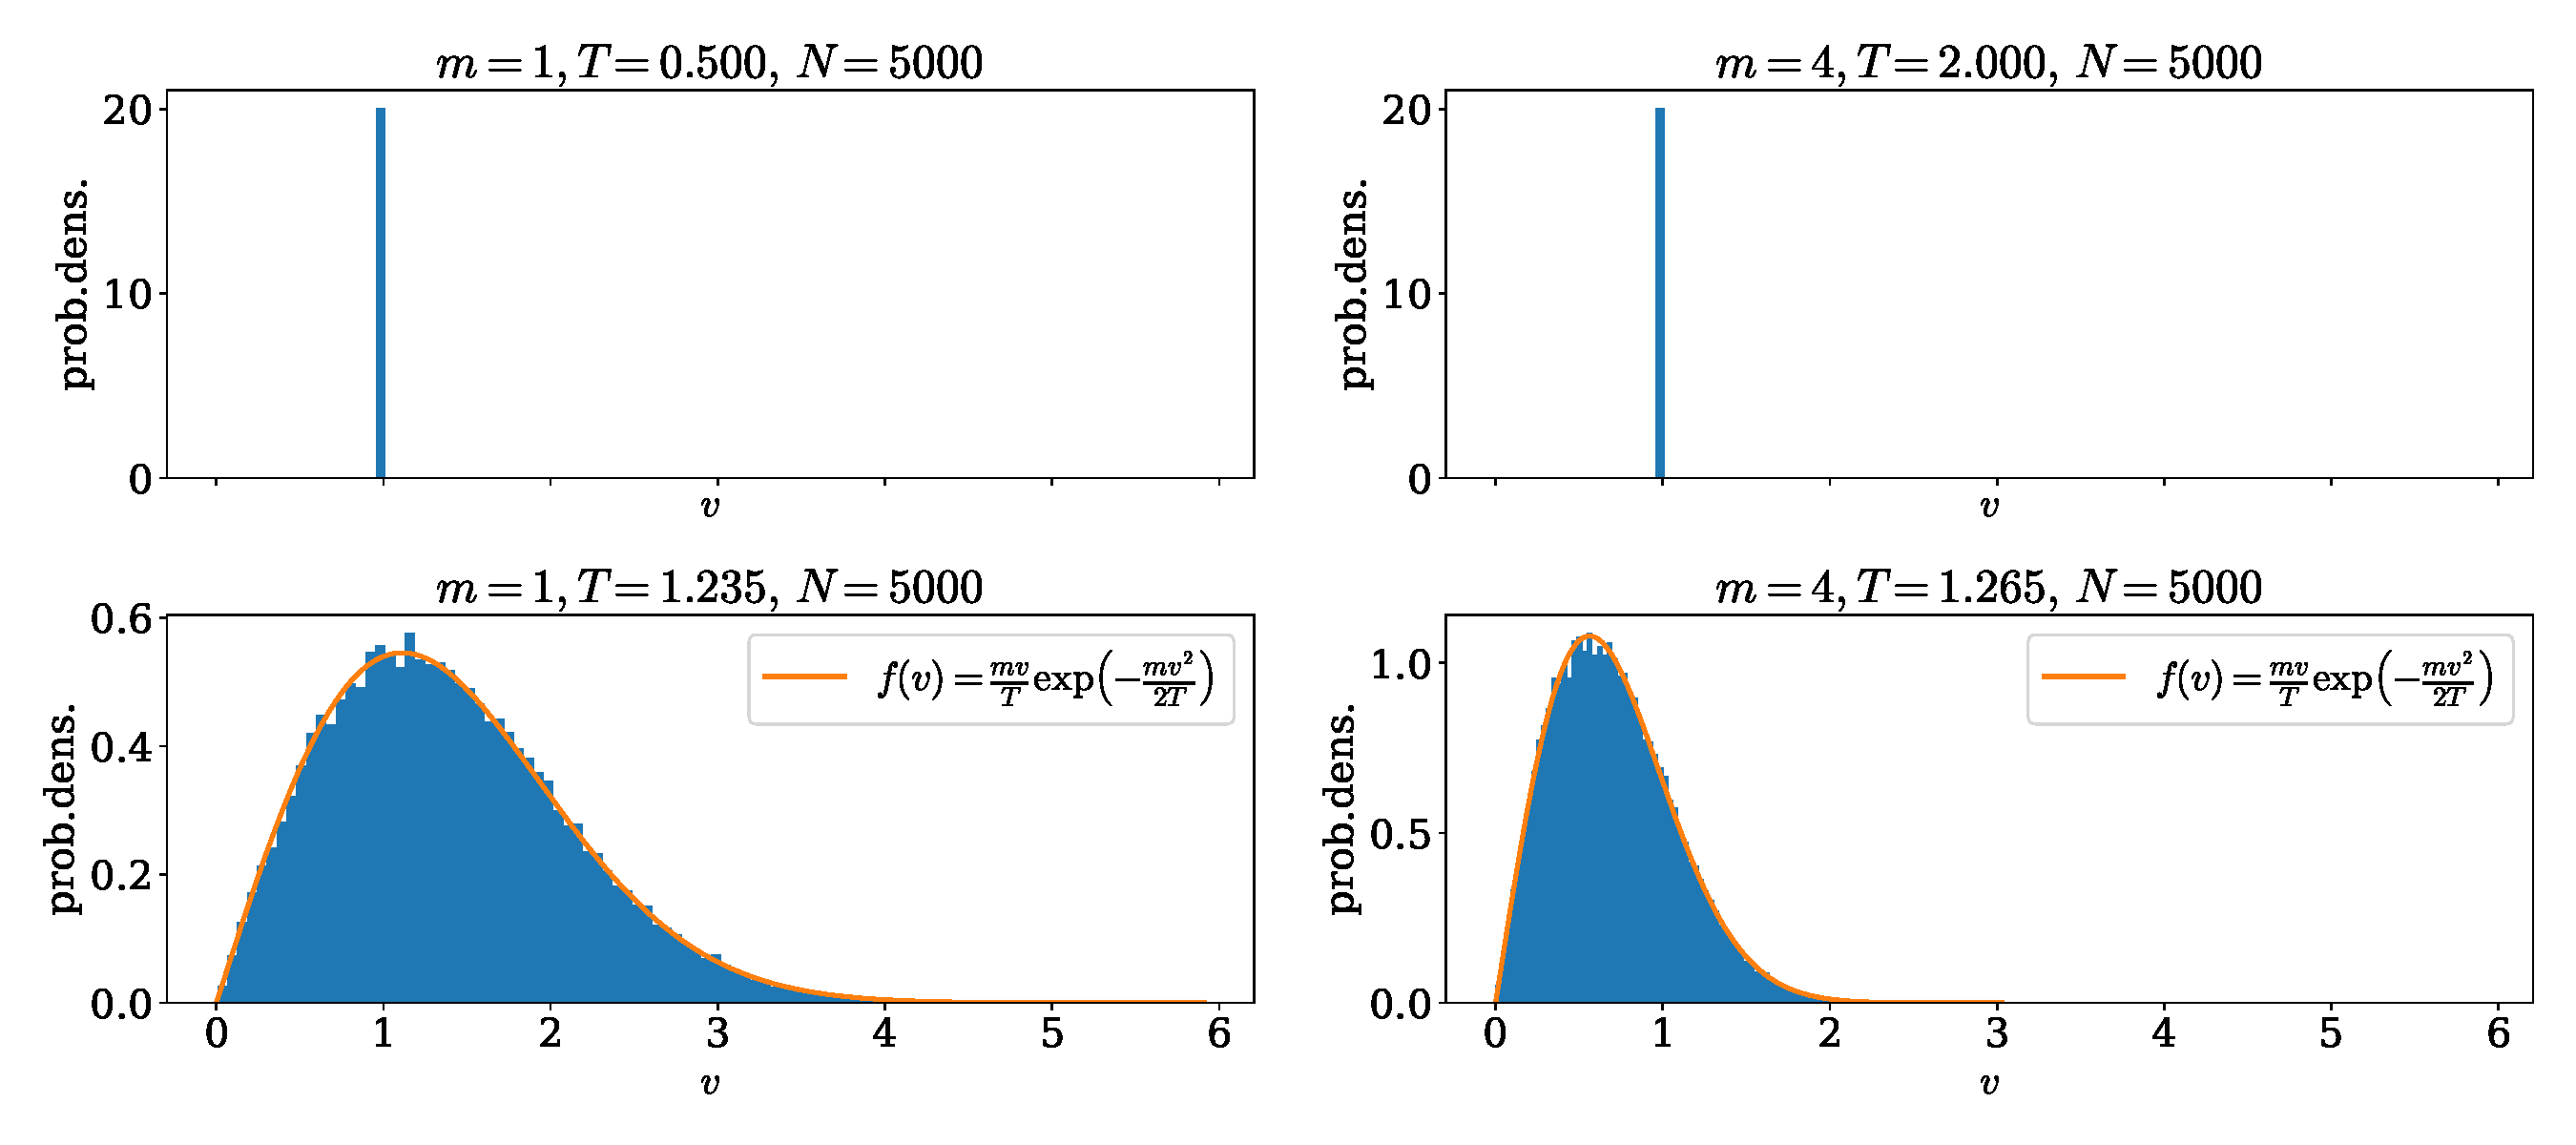
\includegraphics[width=0.9\textwidth]{../plots/problem2/vel_dist.pdf}
        \caption{The velocity distribution of the particles with $m=1$ and $m=4$ is show left and right, resp. and compared to the Maxwell-Boltzmann distribution.}
        \label{problem2 dist}
    \end{figure}
    \begin{figure}[H]
        \centering
        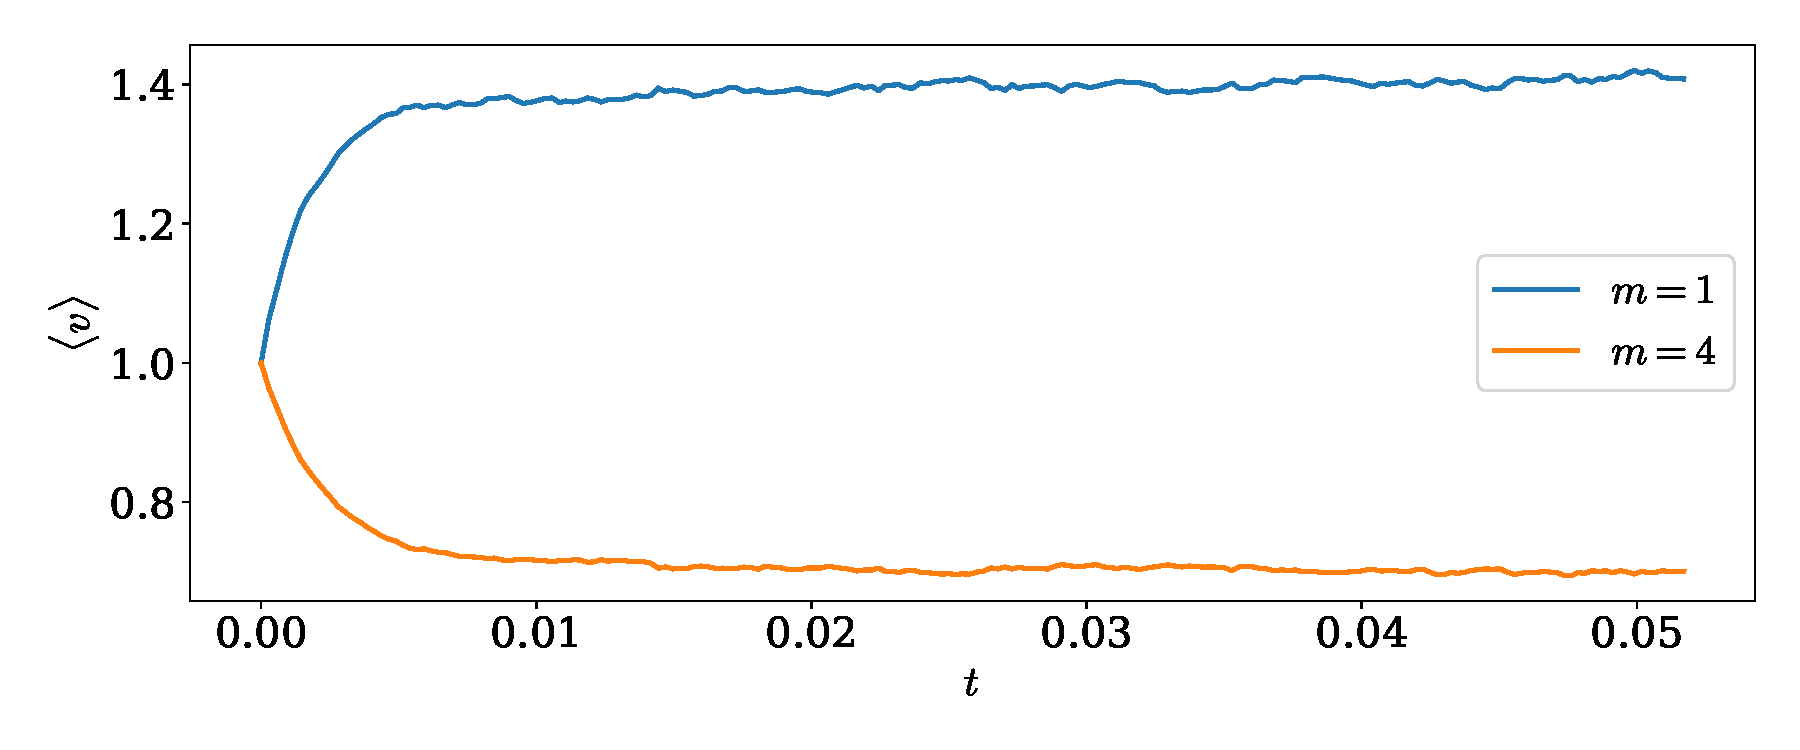
\includegraphics[width=0.7\textwidth]{../plots/problem2/v_av.pdf}
        \caption{The velocity distribution of the particles with $m=1$ and $m=4$ is show left and right, resp. and compared to the Maxwell-Boltzmann distribution.}
        \label{problem2 av vel}
    \end{figure}
    \begin{figure}[H]
        \centering
        \hspace{-5mm}
        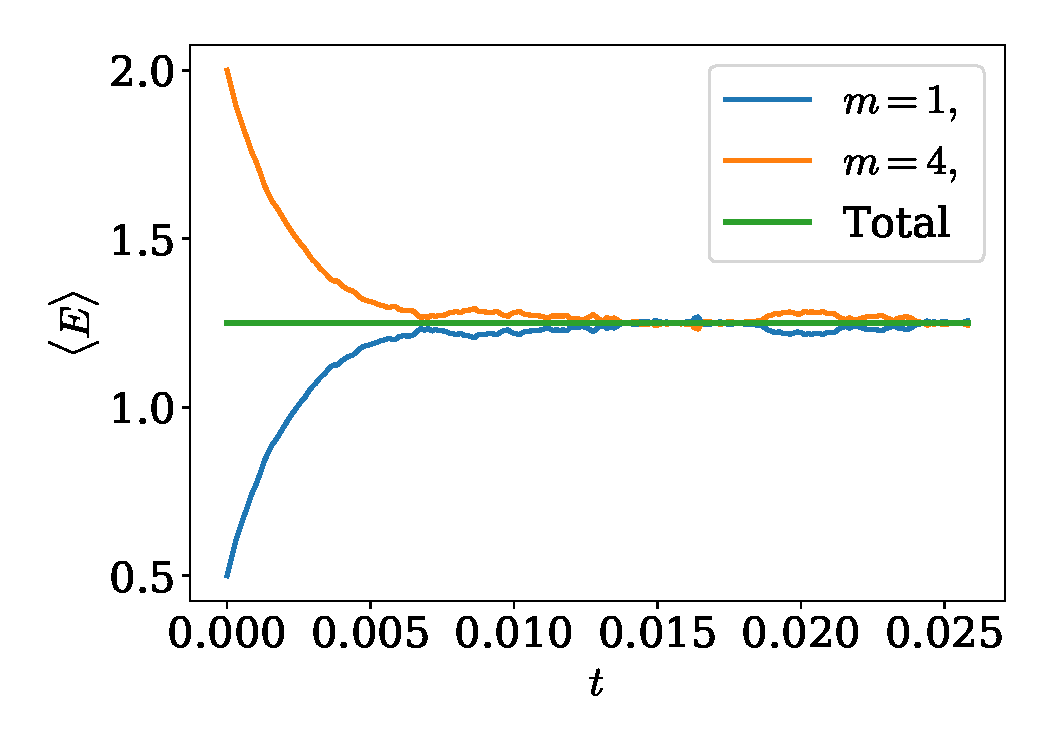
\includegraphics[width=0.35\textwidth]{../plots/problem3/xi_0/energy_ex3.pdf}
        \hspace{-4mm}
        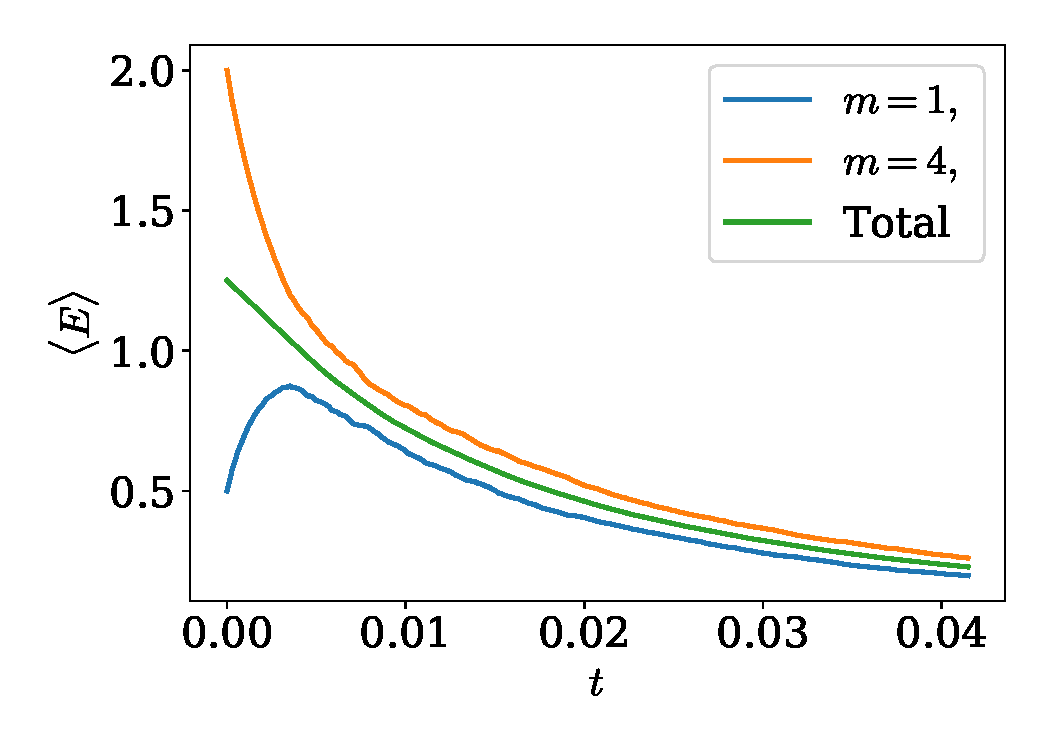
\includegraphics[width=0.35\textwidth]{../plots/problem3/xi_1/energy_ex3.pdf}
        \hspace{-4mm}
        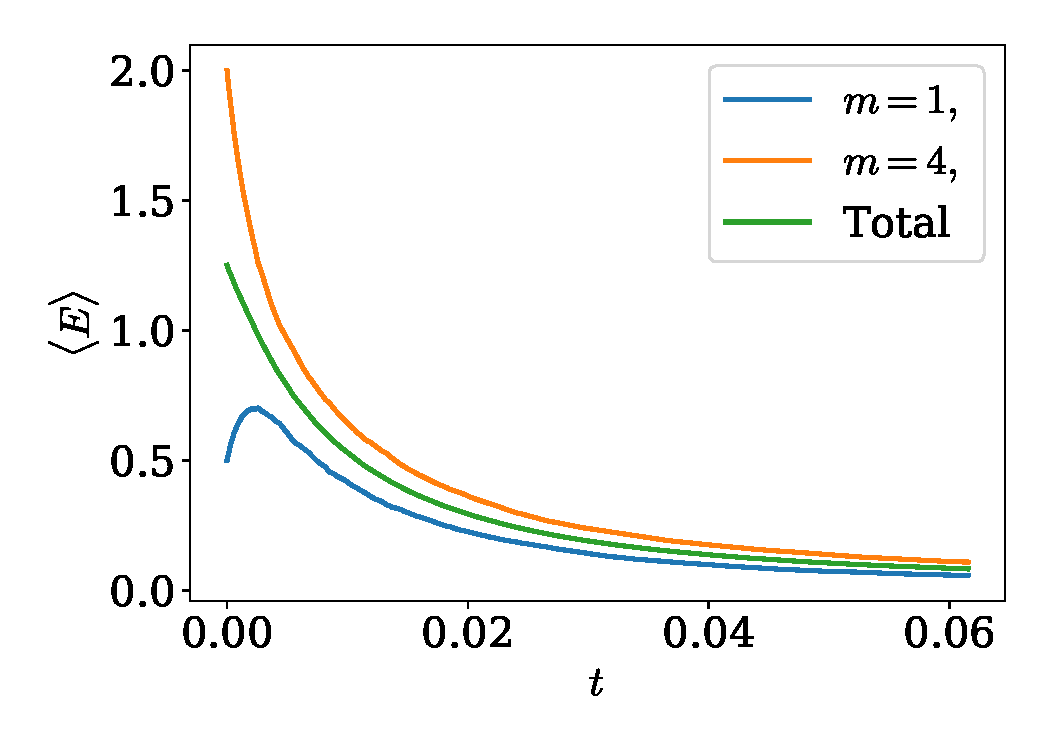
\includegraphics[width=0.35\textwidth]{../plots/problem3/xi_2/energy_ex3.pdf}
        \hspace{-5mm}
        \caption{The average energy, as a function of time, of resp. $\xi=1$, $\xi=0.9$ and $\xi=0.8$.}
        \label{problem2 av en}
    \end{figure}

    \subsection*{Projectile}
    To simulate the impact of a projectile, one particle is placed at $\vec x = (0.5, 0.75)$, and given a velocity of $v = (0, -20)$. The lower half of the square box is filled with small, light particles. The impact from the large disk into the densely packed disks will create a crater. To investigate the effect of the size of projectile on the crater, the simulation is run 10 times, using projectiles with different radius. The crater is measured as described in the implementation section. The mass of the projectile is proportional to $R^2$, so that the density is constant. The simulation uses the value $\xi = 0.5$, and it is run until the total energy of the system is $10\%$ of the original value. There are placed out 2000 particles, of mass radius $R=0.0063$ and mass $R^2$. This means the packing fraction is $2000 \cdot \pi R^2 / 0.5 \approx 0.500$. \autoref{crater size} shows the size of the crater, as a function of the radius of the projectile. The relationship is close to linear.

    \begin{figure}[H]
        \centering
        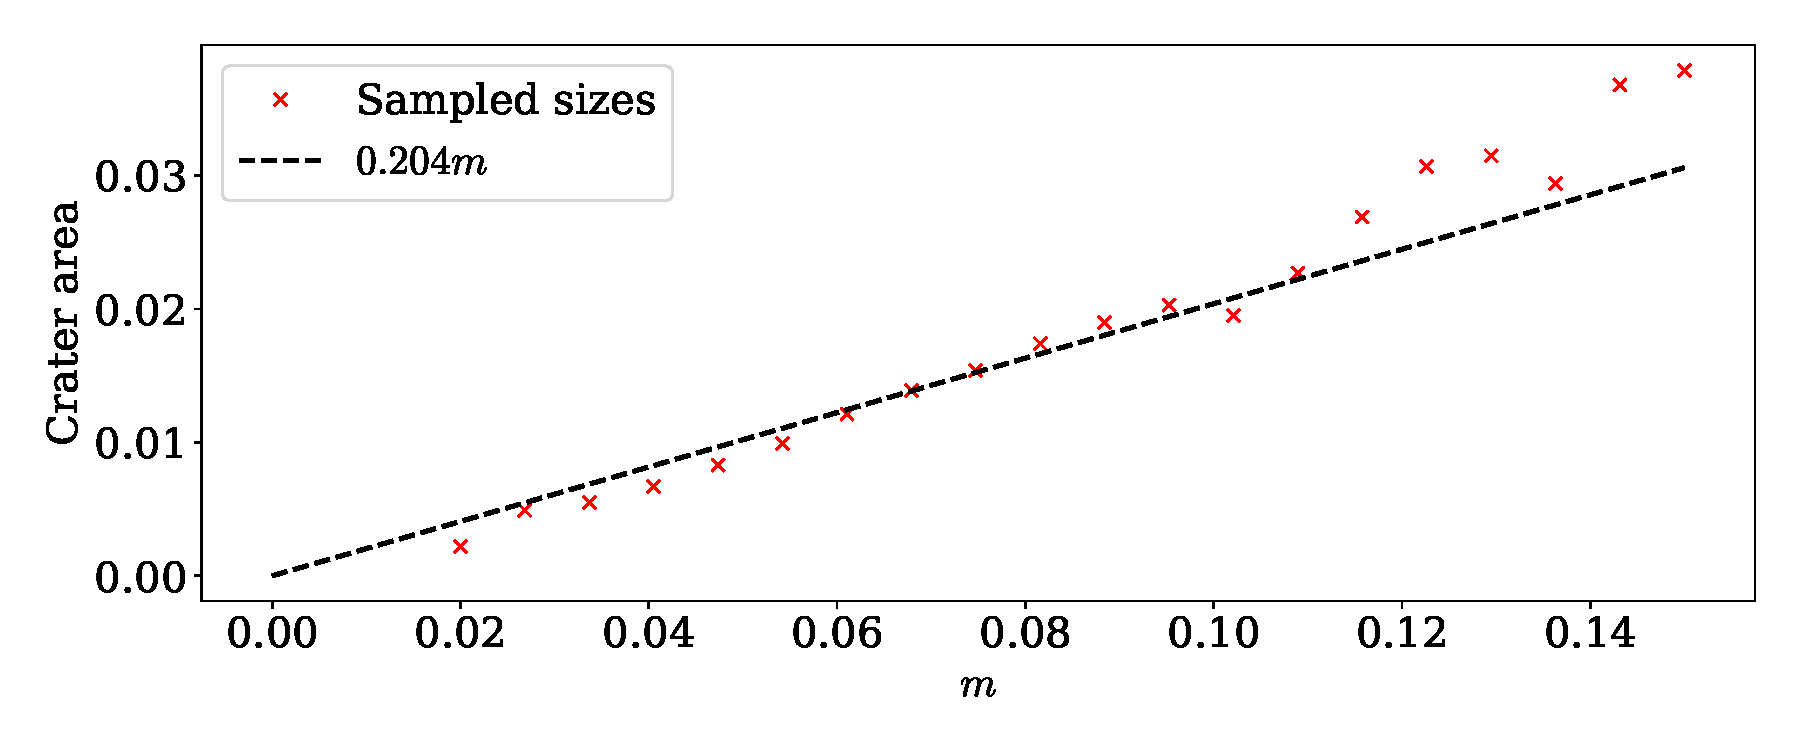
\includegraphics[width=0.7\textwidth]{../plots/problem4/crater_size.pdf}
        \caption{The size of the crater, as a function of the radius of the incoming projectile.}
        \label{crater size}
    \end{figure}

    \section*{Discussion and conclusion}
    The simulation implemented yields accurate results. A good indication of this is how well the energy is conserved, as show by \autoref{test many particles}. The fluctuations here are mostly due to numerical inaccuracies, an negligible for the purposes of these simulations. Discrepancies between the histograms and the Maxwell-Boltzmann distribution comes from the fact that the simulated system is finite, and thus subject to stochastic fluctuations away from perfect equilibrium. The most straight forward way to get better samples would be to simulate more particles, for longer periods of time. At this point, however, the simulation will become increasingly slow, even with the measures taken to speed it up. The larges bottleneck at this time is pushing the collisions to the priority queue. Some measures could be taken to limit this, for example given particle $i$, only push the next collision with, say $j$. Then, if $j$ is involved in another collision, find particle $i$'s next collision. This, however, might lead to a large amount of test reducing the possible gain.
    
    \printbibliography
\end{document}